
\documentclass{beamer}
\usetheme{Electromagnetism}
\usepackage{Electromagnetism}
\graphicspath{{pictures/}}
% -------------------------------------- Grid
%-------------------------------------------------------
\makeatletter
\def\grd@save@target#1{%
  \def\grd@target{#1}}
\def\grd@save@start#1{%
  \def\grd@start{#1}}
\tikzset{
  grid with coordinates/.style={
    to path={%
      \pgfextra{%
        \edef\grd@@target{(\tikztotarget)}%
        \tikz@scan@one@point\grd@save@target\grd@@target\relax
        \edef\grd@@start{(\tikztostart)}%
        \tikz@scan@one@point\grd@save@start\grd@@start\relax
        \draw[minor help lines] (\tikztostart) grid (\tikztotarget);
        \draw[major help lines] (\tikztostart) grid (\tikztotarget);
        \grd@start
        \pgfmathsetmacro{\grd@xa}{\the\pgf@x/1cm}
        \pgfmathsetmacro{\grd@ya}{\the\pgf@y/1cm}
        \grd@target
        \pgfmathsetmacro{\grd@xb}{\the\pgf@x/1cm}
        \pgfmathsetmacro{\grd@yb}{\the\pgf@y/1cm}
        \pgfmathsetmacro{\grd@xc}{\grd@xa + \pgfkeysvalueof{/tikz/grid with coordinates/major step}}
        \pgfmathsetmacro{\grd@yc}{\grd@ya + \pgfkeysvalueof{/tikz/grid with coordinates/major step}}
        \foreach \x in {\grd@xa,\grd@xc,...,\grd@xb}
        \node[anchor=north] at (\x,\grd@ya) {\pgfmathprintnumber{\x}};
        \foreach \y in {\grd@ya,\grd@yc,...,\grd@yb}
        \node[anchor=east] at (\grd@xa,\y) {\pgfmathprintnumber{\y}};
      }
    }
  },
  minor help lines/.style={
    help lines,
    step=\pgfkeysvalueof{/tikz/grid with coordinates/minor step}
  },
  major help lines/.style={
    help lines,
    line width= 0.5pt,
    step=\pgfkeysvalueof{/tikz/grid with coordinates/major step}
  },
  grid with coordinates/.cd,
  minor step/.initial=.2,
  major step/.initial=1,
  major line width/.initial=2pt,
}
\makeatother
\usepackage{cancel}
\begin{document}



%% ============================== Слайд ## ===================================
%\begin{frame}{Гістерезис в діелектриках}{}\small
%\begin{block}{}\justifying
%    \alert{Гістерезис} --- неоднозначна петлеподібна залежність поляризації сегнетоелектриків від
%    зовнішнього електричні поля E за його циклічної зміни.
%\end{block}
%\begin{columns}
%	\begin{column}{0.5\linewidth}\centering
%         \begin{tikzpicture}[>=latex, scale=0.8, transform shape,
%			point/.style={circle, draw, inner sep=0.7pt, fill=white}
%		]
%
%		\draw[-latex, name path=E] (-2.5,0) -- (2.5,0) node[below]{$E$};
%		\draw[-latex, name path
%			=P] (0,-1.5) -- (0,1.5)node[left]{$P$};
%
%		\draw[samples=200, domain=-3:2, name path=d, midarrow,  red, thick] plot ({\x+0.5}, {0.2*\x
%		+ tanh(1.9*\x) + 0.1}); \draw[samples=200, domain=-2:3, name path=u, midarrowR, red, thick]
%		plot ({\x-0.5}, {0.2*\x + tanh(1.9*\x) - 0.1});
%        \draw[midarrow, thick, cyan!50!black] (0,0) .. controls (0.5, 0.2) and
%        (0.2, 1.0) ..
%        (1.52, 1.28);
%		\tikzfillbetween[of=u and d]{blue, opacity=0.1};
%
%		\foreach \i/\a in {P/u, P/d, E/u, E/d} {
%				\path[name intersections={of={\i} and {\a}}]
%				(intersection-1) node[point] (\i\a) {};
%			}
%        \node[left,  text=brown] at (Pu) {$P_r$};
%        \node[right, text=brown] at (Pd) {$-P_r$};
%        \node[above left, text=red] at (Eu) {$-E_c$};
%        \node[below right, text=red] at (Ed) {$E_c$};
%	\end{tikzpicture}
%	\end{column}
%	\begin{column}{0.8\linewidth}
%         \begin{figure}
%            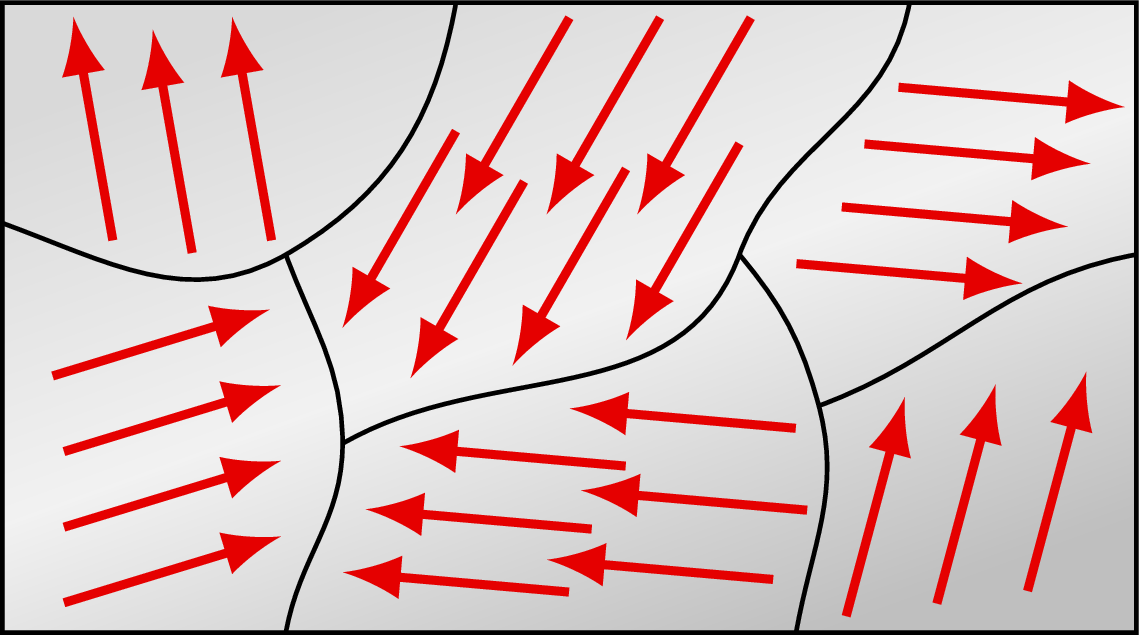
\includegraphics[width=0.5\linewidth]{domains}
%            \caption{\centering\scriptsize Доменна структура сегнетоелектрика}
%        \end{figure}
%	\end{column}
%\end{columns}
%	\begin{enumerate}\justifying\scriptsize
%		\item За високого електричного поля $ E $, поляризація досягає насичення і поводить себе як
%		діелектрик у якого $P \propto E$.
%		\item  Поле зменшується до нуля $E = 0$, але поляризація $ P_r $ залишається.
%		\item Для того щоб звести поляризацію до нуля, потрібно прикласти негативне поле $-E_c$,
%		яке називається \alert{коерцитивною силою}.
%		\item При подальшому збільшенні негативного поля поляризація $P \propto E$.
%		\item  При зменшенні негативного поля до нуля поляризація залишається на рівні $ -P_r $.
%	\end{enumerate}
%\end{frame}
%% ===========================================================================

% ============================== Слайд ## ===================================
\begin{frame}{Підсумки}{}
\begin{tblr}{
colspec={Q[c,l]Q[mode=dmath]}
}
Вектор поляризації & \vect{P} = \frac1V\sum \vect{p}_i \\
Для лінійних діелектриків & \vect{P} = \chi \Efield \\
Теорема Гаусса для вектора $\vect{P}$ & \oiint\limits_S \vect{P}d\vect{S} = - \iiint\limits_V\rho'
dV\\
в диференціальній формі & \divg\vect{P} = - \rho' \\
Вектор електричної індукції & \Dfield = \Efield  + 4\pi\vect{P}\\
Для лінійних діелектриків & \Dfield = \epsilon\Efield \\
{Зв'язок проникності і поляризовності \\ (для лінійних діелектриків)} & \epsilon = 1+ 4\pi\chi \\
Теорема Гаусса в діелектриках & \oiint\limits_S \vect{D}d\vect{S} = 4\pi \iiint\limits_V\rho dV \\
в диференціальній формі & \divg\Dfield = 4\pi\rho
\end{tblr}
\end{frame}
% ===========================================================================

\end{document}